%
% 03_Pitch_Korrektur.tex
%
% (c) 2023 Florian Baumgartner, OST Ostschweizer Fachhochschule
%
% !TEX root = ../../buch.tex
% !TEX encoding = UTF-8
%

\section{Pitch-Korrektur
\label{autotune:section:pitchKorrektur}}
\rhead{Pitch-Korrektur}
Das Ändern der Tonhöhe eines Audiosignals ist keine triviale Aufgabe.
Grundsätzlich ist der Zeit- und Frequenzbereich eines Signals über die Fourier-Transformation miteinander verbunden und kann nicht unabhängig voneinander manipuliert werden.
Dies zeigt der Audruck 
\begin{equation}
    f(t)  \; \laplace \; F(\omega).
\end{equation}
Falls beispielsweise die Tonhöhe eines Audiosignals erhöht werden soll, muss das Audiosignal \glqq schneller\grqq\ abgespielt werden, ähnlich wie bei einer Schallplatte.
Diese Zeitstreckung gillt es jedoch zu vermeiden, da sonst die Dauer der Noten und damit die gesamte Länge der Aufnahme verändert wird.
Algorithmen die die Tonhöhe unabhängig von der Dauer des Audiosignals verändern können, fallen unter den Begriff \textit{Dynamic Time Warping} (DTW).
In der Praxis gibt es eine Vielzahl von Methoden, die sich in ihrer Komplexität und Qualität unterscheiden.
Schlussendlich handelt es sich immer um ein Optimierungsproblem, was für jede Anwendung spezifische Lösungen erfordert.
Wichtig zu erwähnen ist, dass es sich bei allen Algorithmen dieser Art um einen nicht-linearen Prozess handelt,
der verlustbehaftete Resultate liefert.
Im Rahmen dieses Papers wird speziell der Phase Vocoder betrachtet, da er die Grundlage für die meisten Auto-Tune-Algorithmen bildet.


\subsection{Phase Vocoder
\label{autotune:subsection:phaseVocoder}}
\rhead{Phase Vocoder}
Der Phase Vocoder ist ein Algorithmus,
der es ermöglicht die Tonhöhe eines Audiosignals zu ändern, ohne andere Attribute wie die Dauer oder den Klang des Signals negativ zu beeinflussen.
Im Wesentlichen arbeitet der Phase Vocoder,
indem er ein Audiosignal in eine Reihe von überlappenden Fenstern (Frames) zerlegt und anschliessend mithilfe der Fourier-Transformation in den Frequenzbereich umwandelt.
Die Tonhöhenänderung erfolgt dann durch das Skallieren der Frequenzen in der Fourier-Domäne.
Nachdem das Signal im Frequenzbereich manipuliert wurde,
wird es mithilfe der inversen Fourier-Transformation zurück in den Zeitbereich gewandelt.
Dabei wird speziell darauf geachtet, die Phase zwischen benachbarten Fenstern möglichst exakt zu rekonstruieren,
um hörbare Artefakte zu minimieren (siehe \ref{autotune:subsection:fensterRekonstruktion}).
Die Phasenrekonstruktion ist der wesentliche Bestandteil des Phase Vocoder,
woraus sich auch dessen Name ableitet.


\subsection{Spektrum Manipulation
\label{autotune:subsection:spektrumManipulation}}
Im Frequenzbereich kann die Tonhöhe eines Signals durch eine einfache Multiplikation der Frequenzen mittels konstantem Faktor verändert werden.
Die lineare Skallierung wird ausgedrückt als
\begin{equation}
    Y_n(\omega)
    =
    X_n(\omega \cdot R) \;.
\end{equation}
Dabei ist $X_n(\omega)$ das Frequenzspektrum des $n$-ten Fensters und $R$ der Skalierungsfaktor welcher berechnet wird als
\begin{equation}
    R
    =
    \frac{f_{Ref}}{{f_{In}}} \;.
\end{equation}
Wie im Blockschaltbild \ref{autotune:fig:blockschaltbild} erkennbar ist,
stellt $f_{In}$ die gemessene Tonhöhe innerhalb des Fensters dar und $f_{Ref}$ die gewünschte Tonhöhe,
des nächstliegenden Tons aus der Referenz-Tonleiter:
\begin{equation}
    f_{Ref}
    =
    \arg\min_n \left| f_n - f_{In} \right|
    \quad | \quad
    f_n \in [f_{G2}, f_{G\#2}, f_{A2}, ..., f_{F\#4}, f_{G4}] \;.
\end{equation}
Grafisch dargestellt ist diese Skallierung in Abbildung \ref{autotune:fig:spektrumManipulation}.
\begin{figure}
    \centering
    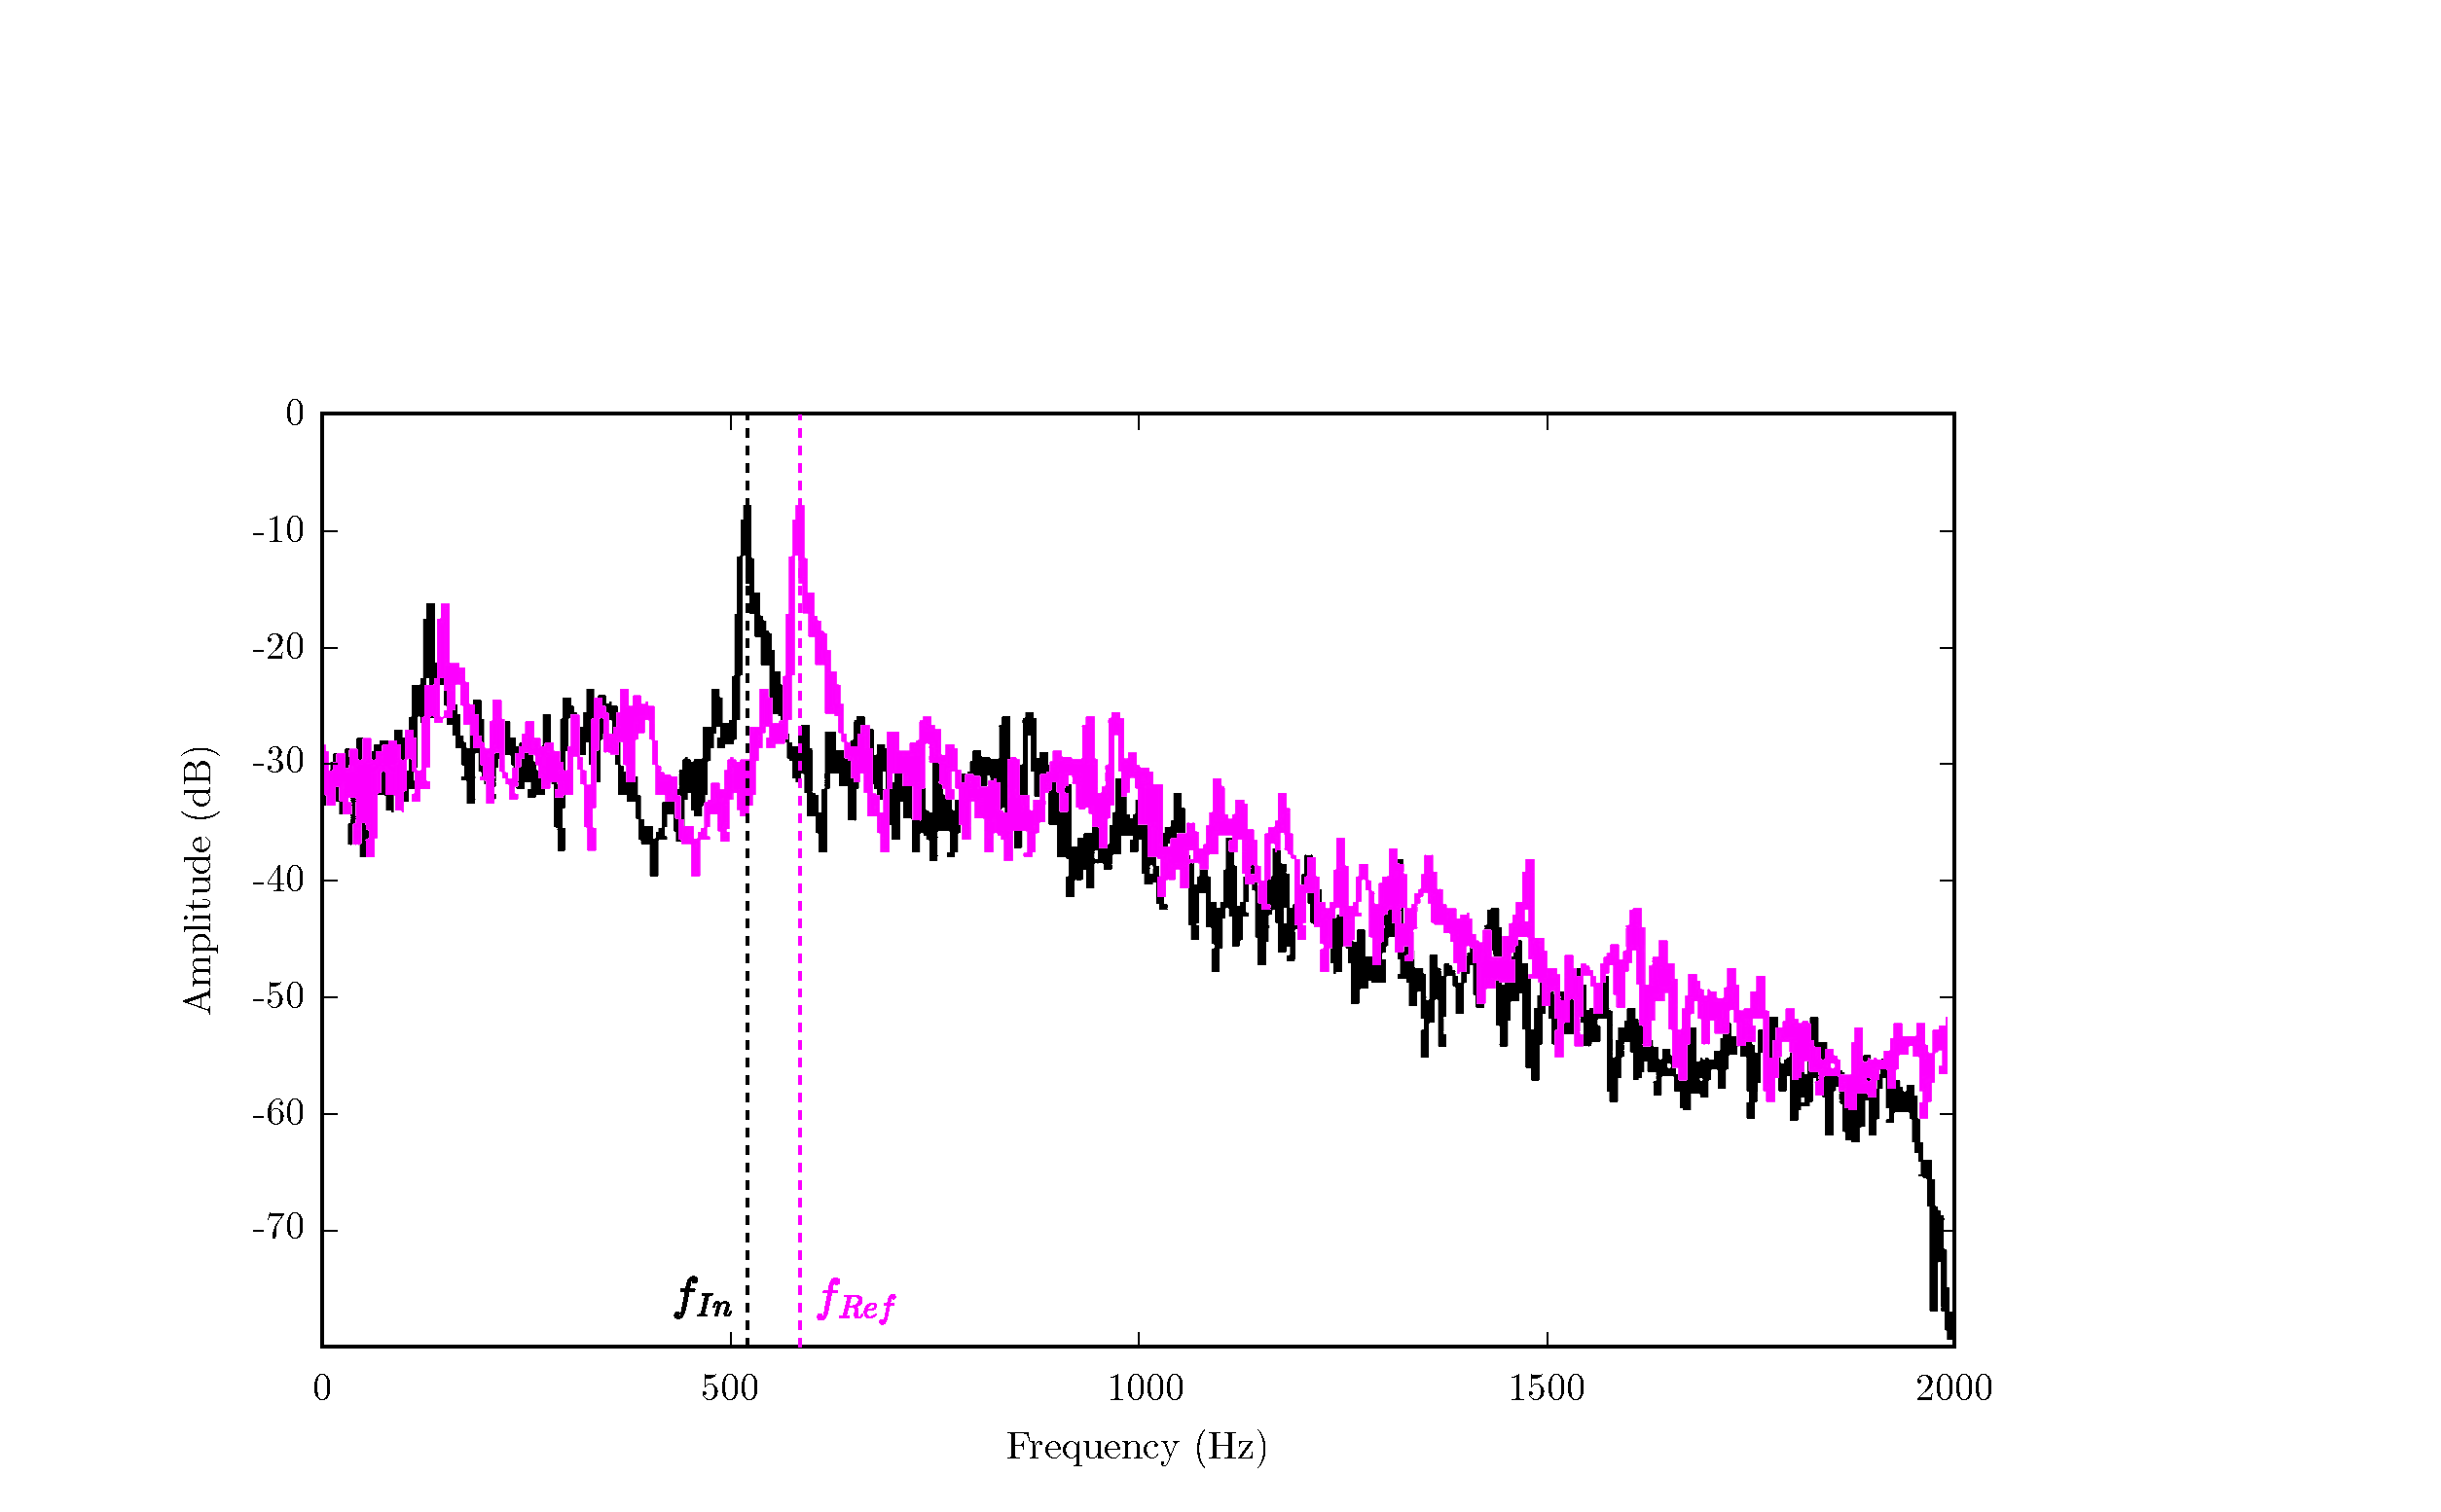
\includegraphics[width=\textwidth]{papers/autotune/images/Spektrum-Manipulation.pdf}
    \caption{Skallierung des Frequenzspektrums}
    \label{autotune:fig:spektrumManipulation}
\end{figure}
Obwohl dieser Ansatz grundsätzlich funktioniert, klingt die resultierende Tonhöhenänderung unnatürlich.
Der entstehende Effekt wird auch als \textit{Chipmunk-Effekt} bezeichnet und ist dafaruf zurückzuführen,
dass die ursprünglichen Formanten des Audiosignals verloren gehen.

%TODO: Add audio example of chipmunk effect

Um den Klangcharakter der menschlichen Stimme beizubehalten,
ist es notwendig das Leistungsdichte-Spektrum möglichst unverändert zu lassen.
Im nächsten Abschnitt \ref{autotune:subsection:formantenErhaltung} wird erläutert, wie dies erreicht werden kann.


\subsection{Formanten Erhaltung
\label{autotune:subsection:formantenErhaltung}}
Formanten sind spezifische Resonanzfrequenzen des menschlichen Vokaltrakts.
Bei der menschlichen Sprachproduktion werden durch die Stimmbänder Schallwellen erzeugt,
die durch den Vokaltrakt (bestehend aus Mund, Nase und Rachen) weiter moduliert werden.
Die Form und Länge des Vokaltrakts bestimmen die Position und Anzahl der Formanten in einem Spektrum. 
Insbesondere sind die ersten beiden Formanten, $F1$ und $F2$,
entscheidend für die Charakterisierung und Unterscheidung von Vokalen.

Die Präsenz der einzelnen Formanten zeigt sich im Leistungsdichte-Spektrum des Audiosignals.
Anders ausgedrückt, representiert die Spektrum-Umhüllende den Klangcharakter, welchen es beim Pitch-Shifting zu erhalten gilt.

In Abbildung \ref{autotune:fig:pitchShiftingSpektrumModellierung} ist dargestellt, wie in der Phase Vocoder ergänzt werden kann,
um die Spektrum-Umhüllende und somit die Formanten zu erhalten.
\begin{figure}
    \centering
    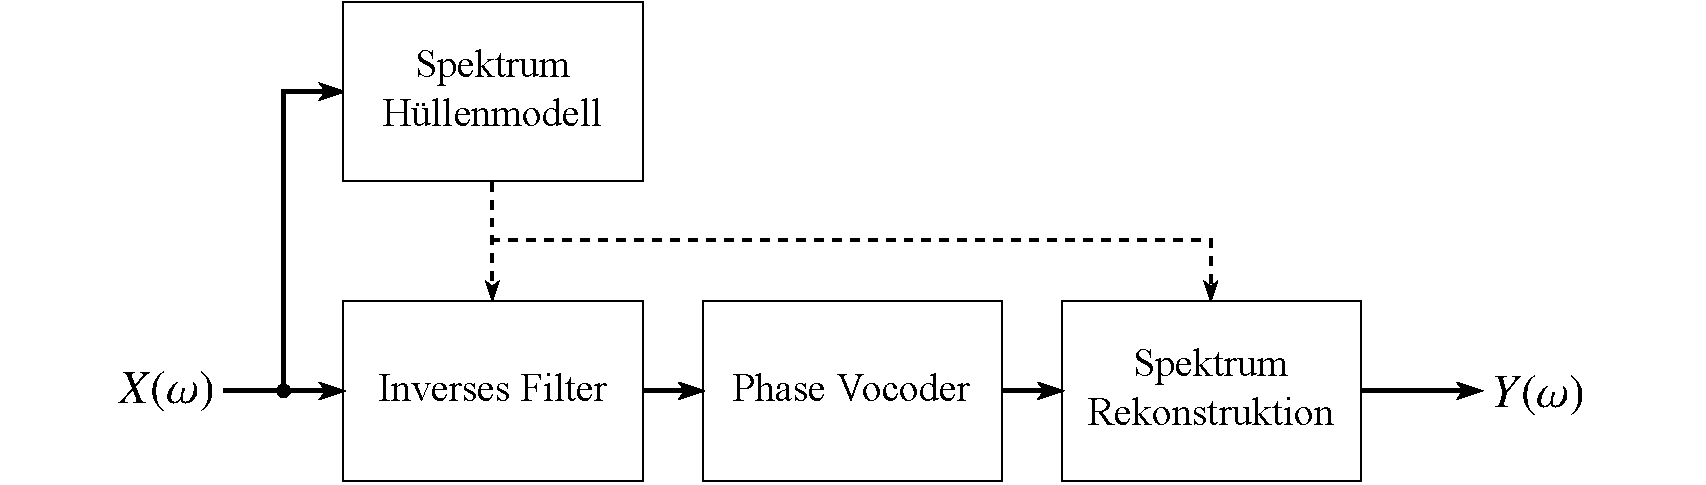
\includegraphics[width=0.9\textwidth]{papers/autotune/images/Spektrum-Modellierung.pdf}
    \caption{Phase Vocoder mit Spektrum-Modellierung}
    \label{autotune:fig:pitchShiftingSpektrumModellierung}
\end{figure}
Als erstes wird die Umhüllende des Spektrums geschätzt.
Diese kann beispielsweise als All-Pol Modell modeliert werden.
Anschliessend wird mittels inversem Filter das Amplitudenspektrum normalisiert (flattening), ausgedrückt als
\begin{equation}
    X_{\text{flat}}(\omega)
    =
    X(\omega) \cdot \frac{1}{\hat{E}_x(\omega)} \;.
\end{equation}
Dabei ist $\hat{E}_x(\omega)$ die geschätzte Umhüllende des Spektrums.
In einem nächsten Schritt wird das Frequenzspektrum skalliert um die gewünschte Tonhöhe zu erreichen.
Zum Schluss folgt die Rekonstruktion der Spektrumumhüllenden mittels zuvor geschätztem All-Pol Modell.
Das resultierende, formantenerhaltende Spektrum ist somit
\begin{equation}
    Y(\omega)
    =
    X_{\text{flat}}(\omega \cdot R) \cdot \hat{E}_x(\omega) \;.
\end{equation}
In Abbildung \ref{autotune:fig:formantenErhaltung} ist der Unterschied zwischen der Spektrum Manipulation mit und ohne Formanten-Erhaltung dargestellt.
\begin{figure}
    \centering
    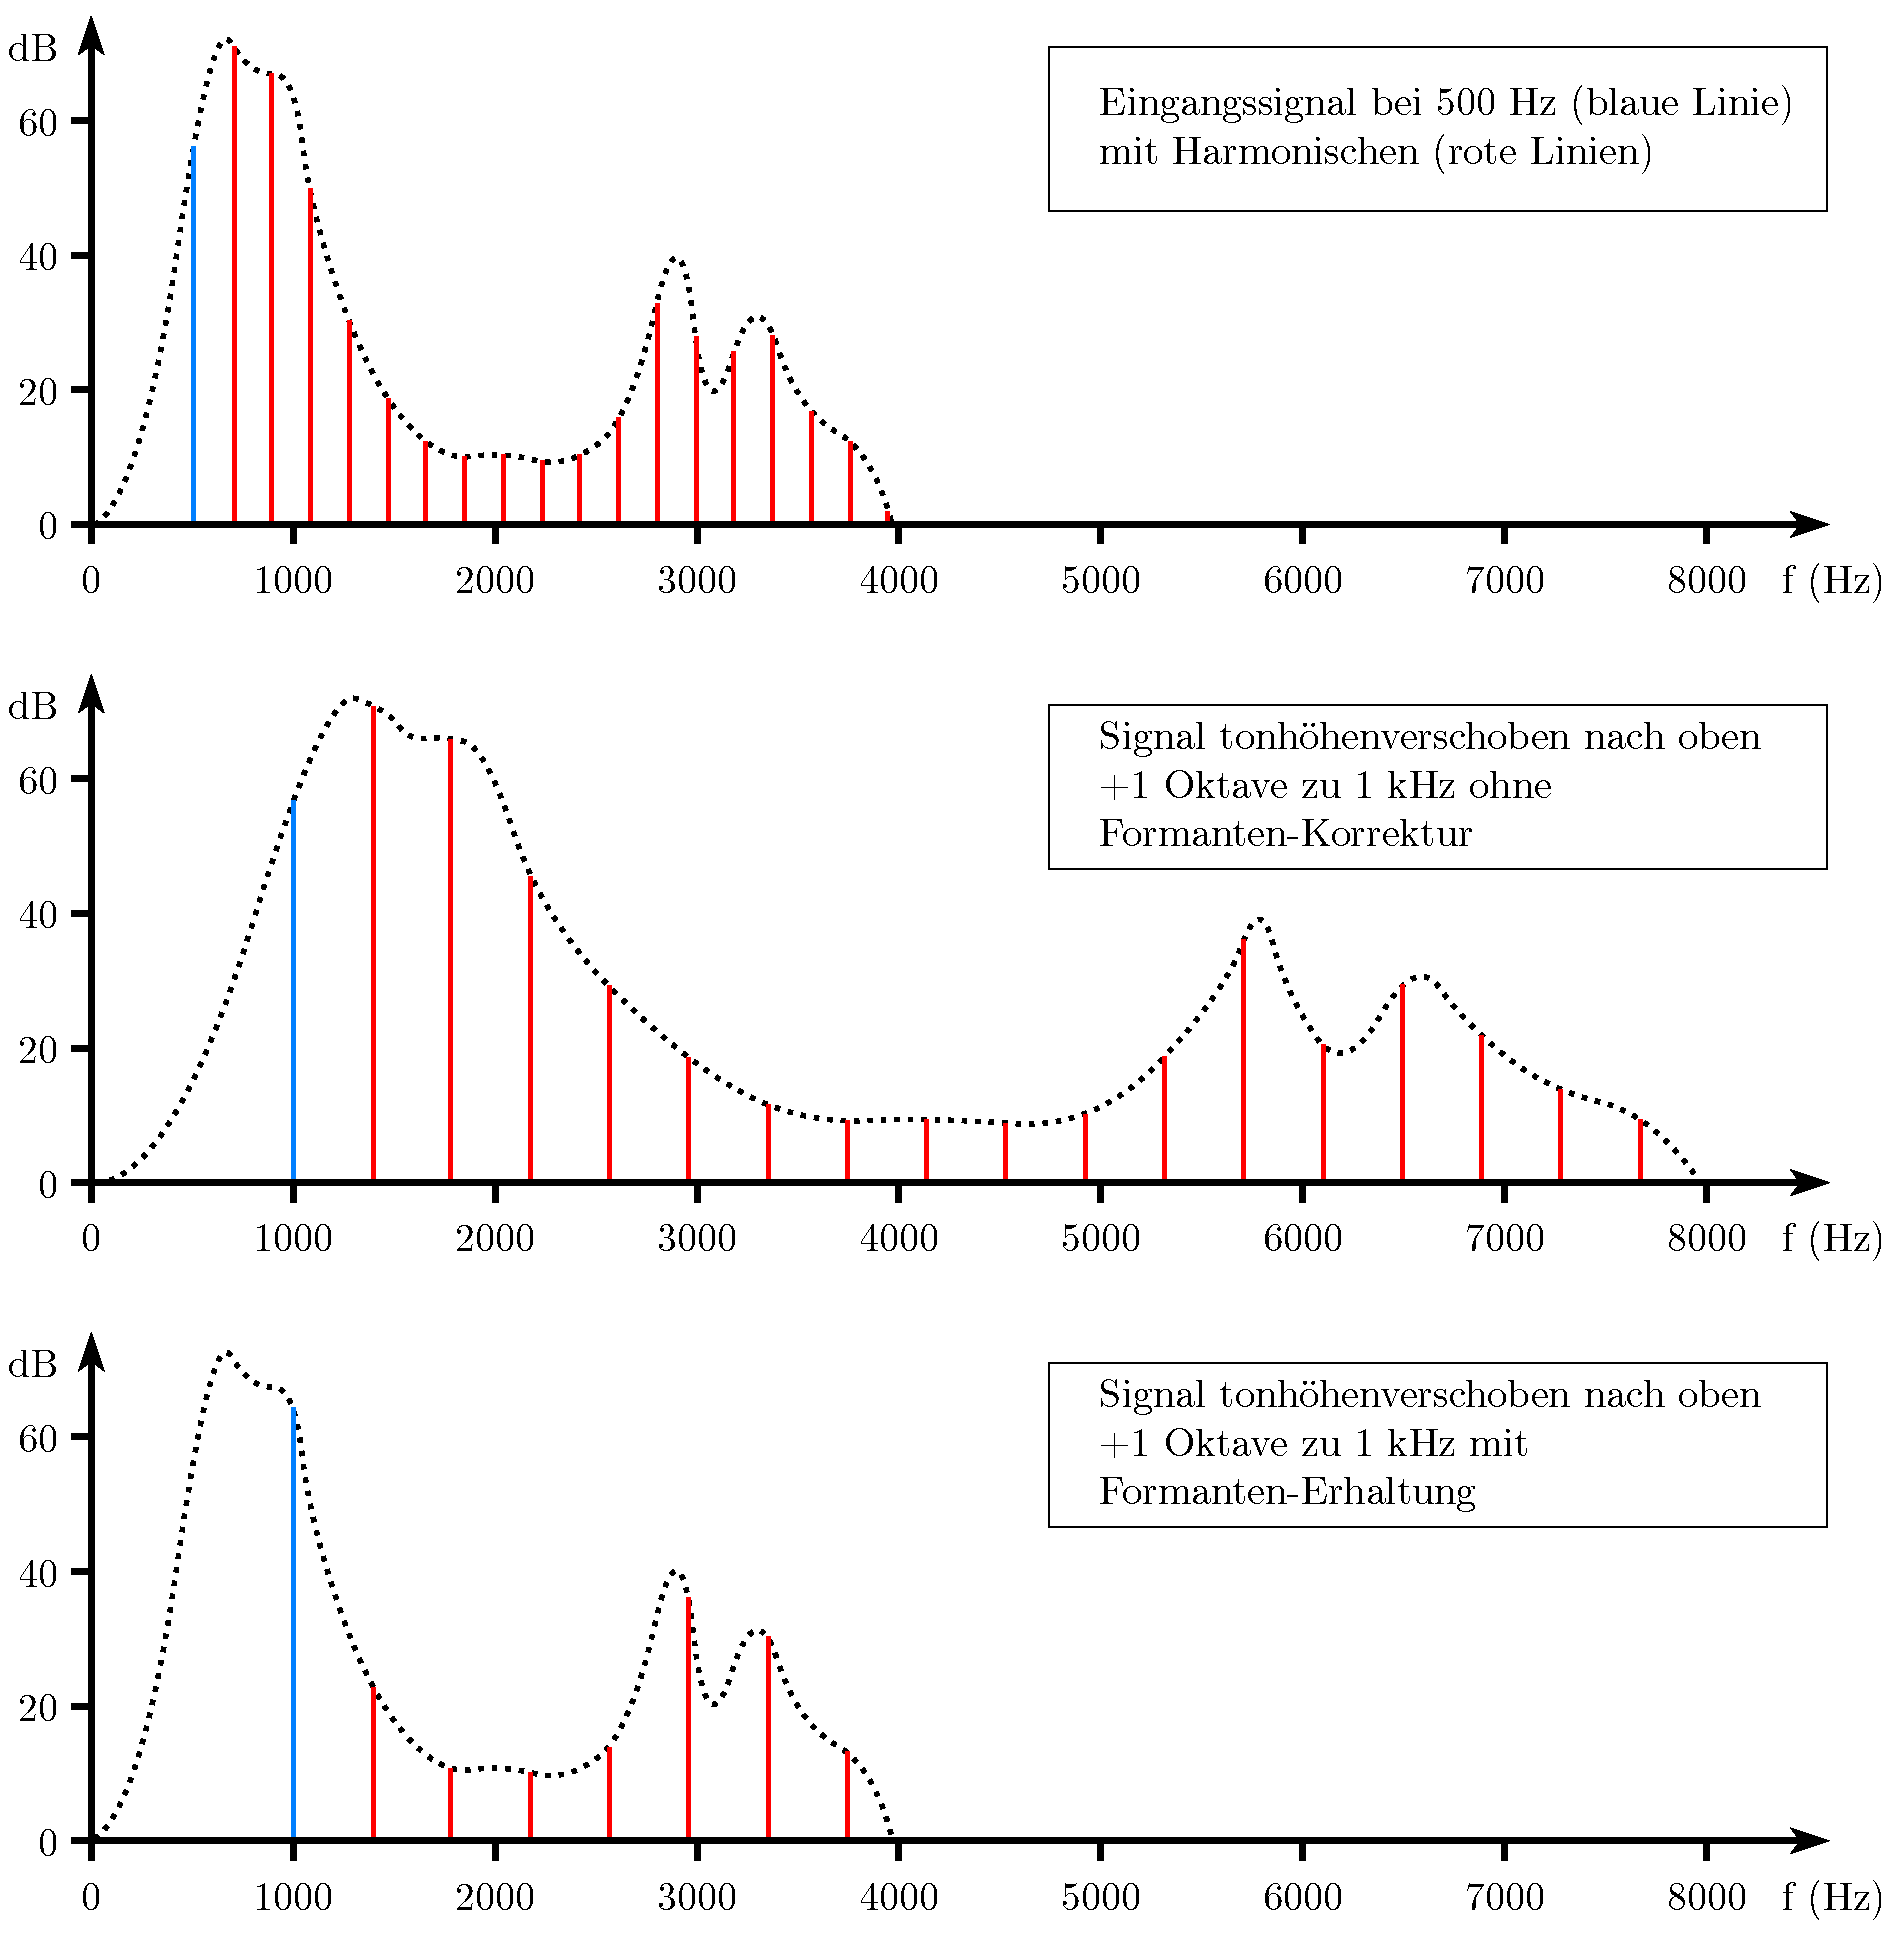
\includegraphics[width=0.95\textwidth]{papers/autotune/images/Formanten-Erhaltung.pdf}
    \caption{Spektrum Manipulation mit und ohne Formanten-Erhaltung}
    \label{autotune:fig:formantenErhaltung}
\end{figure}

% TODO: Add audio example pitch shifting with and without formant preservation


\subsection{Fenster Rekonstruktion
\label{autotune:subsection:fensterRekonstruktion}}
Die Phasenrekonstruktion ist ein wichtiger Bestandteil des Phase Vocoders.
Ziel ist es die Phasensprünge zwischen den Fenstern zu minimieren.
In der Praxis kann dies jedoch nur näherungsweise erfolgen.
Das grundlegende Konzept kann gut anhand eines grafischen Beispiels (Abbildung \ref{autotune:fig:phaseReconstruction}) gezeigt werden.
\begin{figure}
    \centering
    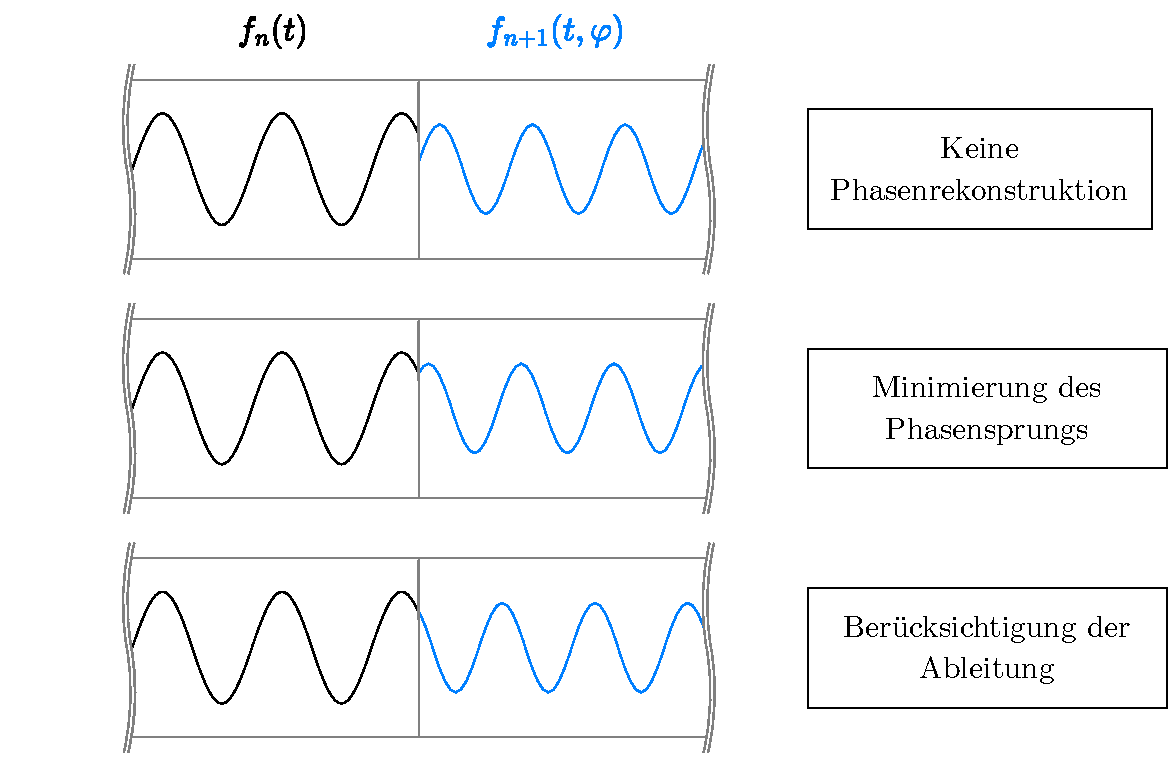
\includegraphics[width=0.8\textwidth]{papers/autotune/images/Fenster-Rekonstruktion.pdf}
    \caption{Fenster Rekonstruktion mit und ohne Berücksichtigung der Phasen}
    \label{autotune:fig:phaseReconstruction}
\end{figure}

Gegeben seien die Fenster als Funtionen $f_n(t)$ und $f_{n+1}(t, \varphi)$.
Sie sind das Resultat der inversen Short-Time-Fouriertransformation $\textbf{ISTFT}$ des manipulierten Spektrums,
ausgedrückt als
\begin{equation}
    \begin{aligned}
        f_n(t)
        &=
        \sum_{\omega} X(n, \omega) e^{j\omega t} w(t - n) \\
        f_{n+1}(t, \varphi)
        &=
        \sum_{\omega} X(n+1, \omega) e^{j(\omega t + \varphi)} w(t - (n+1)) \;.
    \end{aligned}
\end{equation}
Es gillt nun also die Phasenverschiebung $\varphi$ des nachfolgenden Fensters $f_{n+1}$ so zu wählen,
dass die Differenz zwischen dem vorherigen Fenster $f_n$ zum Zeitpunkt $t_0$ (Überlappungszeitpunkt) minimal wird.
Des weiteren gillt es zu beachten, dass zusätzlich auch die Vorzeichen der Ableitungen $\dot{f}_n$ und $\dot{f}_{n+1}$ übereinstimmen müssen,
um einen monotomen Übergang zwischen den Fenstern zu gewährleisten.
Das Optimierungsproblem kann wie folgt formuliert werden:
\begin{equation}
    \begin{aligned}
        \underset{\varphi \; \in \; \mathbb{R}}{\text{minimize}}
        & \quad
        \Delta f(t=t_0, \varphi) = |f_n(t) - f_{n + 1}(t, \varphi)| \\
        \text{subject to}
        & \quad
        \text{sign}(\dot{f}_n(t_0)) \stackrel{!}{=} \text{sign}(\dot{f}_{n + 1}(t_0, \varphi)) \\
        & \quad
        0 \leq \varphi < 2\pi \;.
    \end{aligned}
\end{equation}
In der Praxis wird oft mit einem Überlappungsfaktor zwischen den Fenstern gearbeitet, der die Phasensprünge weiter reduziert (Stichwort Overlap-Add).
Bei guter Umsetzung dieses Verfahren kann die Qualität der rekonstruierten Audiosignale stark verbessert werden.
Ansonsten können hörbare Artefakte entstehen, welche sich beispielsweise als \glqq metallischer Klang\grqq\ oder erhöhtes Rauschen äussern.

% TODO: Add audio examples of baddly and well reconstructed frames
